\begin{frame}{Motivation}
    \begin{center}
        \begin{center}
            \Large
            Rechnen mit unendlich vielen Zahlen ist hart
        \end{center} 
        \pause
        \vspace{1cm}

        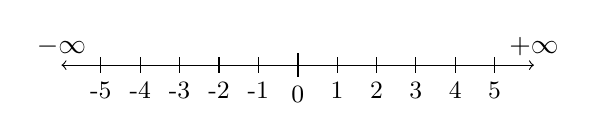
\begin{tikzpicture}[x=.5cm,y=1cm]

            % The number line with arrows on both ends
            \draw[<->] (-6,0) -- (6,0);

            % Infinity hints
            \node[above] at (-6,0) {$-\infty$};
            \node[above] at (6,0) {$+\infty$};

            % Tick marks (loop)
            \foreach \x in {-5,-4,...,5}
                \draw (\x,0.1) -- (\x,-0.1);

            % Labels for nonzero ticks (loop)
            \foreach \x in {-5,-4,...,-1,1,2,...,5}
                \node[below] at (\x,-0.1) {\small \x};

            % Thicker tick and label for zero
            \draw[thick] (0,0.15) -- (0,-0.15);
            \node[below] at (0,-0.15) {\small 0};

        \end{tikzpicture}
    \end{center}
\end{frame}

\begin{frame}{Motivation}
    \begin{center}
        \begin{center}
            \Large
            Wir können einfach nur mit den Zahlen $0$ bis $5$ rechnen
        \end{center} 
        \pause
        \vspace{1cm}

        \begin{tikzpicture}[x=.5cm,y=1cm]

            % The number line with arrows on both ends
            \draw[-] (-6,0) -- (6,0);

            % Tick marks (loop)
            \foreach \x in {0,...,5}
                \draw (\x,0.1) -- (\x,-0.1);

            % Labels for nonzero ticks (loop)
            \foreach \x in {1,2,...,5}
                \node[below] at (\x,-0.1) {\small \x};

            % Thicker tick and label for zero
            \draw[thick] (0,0.15) -- (0,-0.15);
            \node[below] at (0,-0.15) {\small 0};

        \end{tikzpicture}
    \end{center}
    \pause
        \begin{center}
            \Large
            Was ist jetzt $3+4$?
        \end{center} 
\end{frame}

\begin{frame}[fragile]{Motivation}
    \begin{center}
        \vspace{1cm}

        \begin{tikzpicture}[x=1cm,y=1cm]

            % Draw the circle
            \draw (0,0) circle (2);

            % Place the numbers 0 to 5 equally spaced
            \foreach \i in {0,...,5} {
                \node[font=\small] at ({-60*(\i-1)}:2.2) (\i){\i}; % labels slightly outside
                \draw[-] ({60*\i}:1.9) to ({60*\i}:2.1);
            }

            \pause
            \draw[->, in = -180, out = -120] (3) to (4);
            \draw[->, in = -240, out = -180] (4) to (5);
            \draw[->, in = -300, out = -240] (5) to (0);
            \draw[->, in = -360, out = -300] (0) to (1);
    
            

        \end{tikzpicture}
    \end{center}
\end{frame}

\begin{frame}[fragile]{Modulo}
    \begin{center}
        \Large
        $$
        3+4 \equiv 1 \mod 6
        $$

        \pause
        Das bedeutet so viel wie:
        $$
        (3+4)\% 6 = 1 \% 6
        $$
    \end{center}
\end{frame}


\begin{frame}[fragile]{Restklassenring}
    \begin{itemize}
        \item Wir nennen so einen begrenzten Zahlenraum \alert{Restklassenring}
        \item Die mathematische Schreibweise für einen Restklassenring mit $m$ Zahlen ist:
        $$
        \mathbb Z / m\mathbb Z
        $$
    \end{itemize}
\end{frame}

{\setbeamercolor{palette primary}{bg=ExColor}
\begin{frame}[fragile]{Denkpause}
    \footnotesize
        \begin{alertblock}{Aufgaben}
        \end{alertblock}
        \metroset{block=fill}
        \begin{block}{löst die folgenden Rechenaufgaben im $\mathbb Z/12\mathbb Z$}
            \begin{multicols}{3}
            \begin{itemize}
                \item $10 + 2$
                \item $3\cdot4-1$
                \item $(2-4)2$
            \end{itemize}
            \end{multicols}
        \end{block}
        \begin{block}{löst die folgenden Rechenaufgaben im $\mathbb Z/7\mathbb Z$}
            \begin{multicols}{3}
            \begin{itemize}
                \item $5 + 1$
                \item $3\cdot4-1$
                \item $(2-4)2+5$
                \item $5^2$
                \item $0\cdot4$
                \item $5!$
            \end{itemize}
            \end{multicols}
        \end{block}
        \begin{block}{Was ist $m$?}
            \begin{multicols}{3}
            \begin{itemize}
                \item $4 \equiv 6 \mod m$
                \item $3 \equiv 9 \mod m$
                \item $4 \equiv 11 \mod m$
            \end{itemize}
            \end{multicols}
        \end{block}
\end{frame}

\begin{frame}<handout:0>{Lösungen}
  \begin{itemize}[<+- | alert@+>]
        \item $10+2 \equiv 0 \mod 12$
        \item $3\cdot 4-1 \equiv 11 \mod 12$
        \item 
        \begin{align*}
        (2-4)2 &\equiv x \mod 12\\
        (-2)2 &\equiv x \mod 12\\
        -4 &\equiv x \mod 12\\
        12-4&=8
        \end{align*}

        oder
        \begin{align*}
        (2-4)2 &\equiv x \mod 12\\
        (-2)2 &\equiv x \mod 12\\
        (10)2 &\equiv x \mod 12\\
        20 &\equiv x \mod 12\\
        20-12 &= 8 
        \end{align*}
    \end{itemize}
\end{frame}

\begin{frame}<handout:0>{Lösungen}
  \begin{itemize}[<+- | alert@+>]
                \item $5 + 1      \equiv 6 \mod 7$
                \item $3\cdot4-1  \equiv 4 \mod 7$
                \item $(2-4)2+5   \equiv 1 \mod 7$
                \item $5^2        \equiv 4 \mod 7$
                \item $0\cdot4    \equiv 0 \mod 7$
                \item $5!         \equiv 1 \mod 7$
    \end{itemize}
\end{frame}

\begin{frame}<handout:0>{Lösungen}
  \begin{itemize}[<+- | alert@+>]
                \item $4 \equiv 6 \mod m$
                
                $m \in \{1,2\}$
                \item $3 \equiv 9 \mod m$

                $m \in \{1,3\}$
                \item $4 \equiv 11 \mod m$

                $m \in \{1,7\}$
    \end{itemize}
\end{frame}
}

\begin{frame}{Wofür brauchen wir das?}
    \begin{outline}
        \1 Computer sind nicht unendlich groß
            \2 Variablen verbrauchen eine fixe Menge Platz
            \2 Was machen wenn die Zahl zu groß wird für diesen Platz?
            \2 Z.B. der unsigned Integer ist im $\mathbb Z / 2^{64}\mathbb Z$
            \pause
        \1 Hashing / Checksums
            \2 Wie stelle ich sicher ob eine Datei die Datei ist, die ich haben will?
            \pause
        \1 Verschlüsselung
            \2 Moderne Kryptographie verwendet die modulare Arithmetik 

    \end{outline}
\end{frame}

{\setbeamercolor{palette primary}{bg=ExColor}
\begin{frame}[fragile]{Knobelaufgabe}
    \footnotesize
        \metroset{block=fill}
        \begin{block}{Finde eine Zahl $n \in \mathbb N$ für die alle folgenden Eigenschaften gelten:}
            \begin{multicols}{2}
            \begin{itemize}
                \item $n \equiv m \mod 2$
                \item $m \in \{2x | x \in \mathbb N\}$
                \item $n \equiv k \mod 17$
                \item  $\exists x: m-x < 0 \wedge m\cdot x < 100$
            \end{itemize}
            \end{multicols}
        \end{block}
        
\end{frame}

}